\documentclass[10pt]{article}

\usepackage{geometry}
\geometry{margin = 1in,top =0.12\paperheight, headheight=\paperheight}
\usepackage[export]{adjustbox}
\usepackage{array}
\usepackage{amsmath}
\usepackage{amsfonts}
\usepackage{fancyhdr}
\usepackage{lastpage}
\usepackage{xcolor}
\pagestyle{fancy}
\fancyhf{}
\rhead{Written Assignment, Page \thepage}
\lhead{MATH211}
\chead{
\includegraphics[width = 0.15\textwidth]{MCLogo-Bck.png}}


%\renewcommand{\footrulewidth}{0.4pt}

\usepackage{enumitem}
\usepackage{pifont}
\usepackage{graphicx}
\graphicspath{{../img}}

\newtheorem{theorem}{Theorem}
\newtheorem{exercise}{Exercise}


\newcommand{\R}{\mathbb R}
\newcommand{\e}{{\rm e}}
\newcommand{\inpr}[1]{\left\langle#1\right\rangle}
\newcommand{\norm}[1]{\lVert #1 \rVert}
\newcommand{\abs}[1]{\lvert #1 \rvert}
\newcommand{\vv}{\mathbf v}
\newcommand{\uv}{\mathbf u}

\DeclareMathOperator{\xd}{d\!}
\DeclareMathOperator{\proj}{proj}

\title{}
\date{}

\begin{document}
\noindent {\bf Problem.}
Consider $\displaystyle \lim_{(x,y)\to(0,0)}\frac{x^2y}{x^4+y^2}$.
\begin{enumerate}[label = (\alph*)]
\item Determine the path limit at $(0,0)$ along all straight paths. (Hint: Different straight paths have different algebraic expressions. Therefore, you have to deal with {\bf three} categories (NOT three concrete examples.))
\begin{figure}[h]
\begin{flushright}
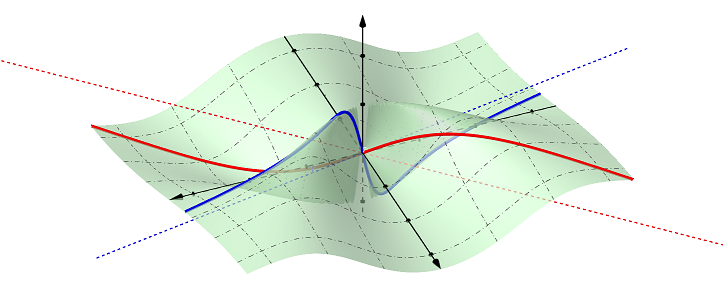
\includegraphics[width=0.35\textwidth]{function4.png}
\end{flushright}
\end{figure}
\vspace{\stretch{2}}

\item Determine the path limit at $(0,0)$ along the parabolic path $y=x^2$.
\begin{figure}[h]
\begin{flushright}
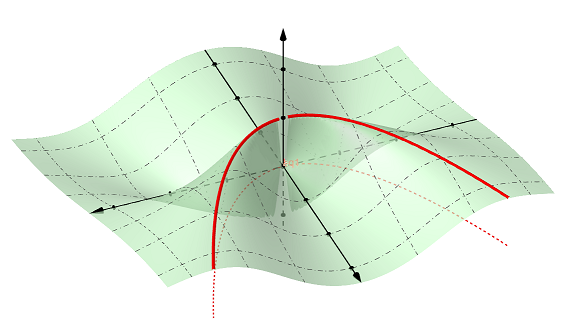
\includegraphics[width=0.3\textwidth]{function5.png}
\end{flushright}
\end{figure}
\vspace{\stretch{1}}

\item Dose the (overall) limit exist? Type your explanation. ({\bf Remark.} Handwritten response receives no credit for this part.)
\end{enumerate}
\clearpage

\end{document}